\documentclass[pdflatex,compress,mathserif]{beamer}

%\usetheme[dark,framenumber,totalframenumber]{ElektroITK}
\usetheme[darktitle,framenumber,totalframenumber]{ElektroITK}

\usepackage[utf8]{inputenc}
\usepackage[T1]{fontenc}
\usepackage{lmodern}
\usepackage[bahasai]{babel}
\usepackage{amsmath}
\usepackage{amsfonts}
\usepackage{amssymb}
\usepackage{graphicx}
\usepackage{multicol}
\usepackage{lipsum}

\newcommand*{\Scale}[2][4]{\scalebox{#1}{$#2$}}%

\title{METODE NUMERIK}
\subtitle{Regresi}

\author{Tim Dosen Pengampu}

\begin{document}

\maketitle

\section{Sub-CMPK dan Bahan Kajian}

\begin{frame}
	\frametitle{Sub-CMPK dan Bahan Kajian}
	\begin{itemize}
		\item \textbf{Sub-CPMK:} Mahasiswa mampu melakukan regresi numerik
		\item \textbf{Bahan Kajian:}
		\begin{enumerate}
			\item Regresi Lanjar
			\item Pelanjaran
		\end{enumerate}
	\end{itemize}
\end{frame}

\section{Pendahuluan}

\begin{frame}
	\frametitle{Pendahuluan}
	\begin{itemize}
		\item Regresi adalah teknik pencocokan kurva untuk data yang
berketelitian rendah.
		\item Contoh data yang berketelitian rendah data hasil pengamatan, percobaan di laboratorium, atau data statistik. Data seperti itu kita
sebut data hasil pengukuran.
		\item Untuk data hasil pengukuran, pencocokan kurva berarti membuat
fungsi mengampiri (approximate) titik-titik data.
		\item Kurva fungsi hampiran tidak perlu melalui semua titik data tetapi
dekat dengannya tanpa perlu menggunakan polinom berderajat
tinggi.
	\end{itemize}
\end{frame}

\begin{frame}
	\begin{itemize}
		\item \textbf{Contoh:} diberikan data jarak tempuh ($ y $) sebuah kendaraaan -dalam mil- setelah $ x $ bulan seperti pada tabel di bawah ini
	\end{itemize}
	\begin{center}
		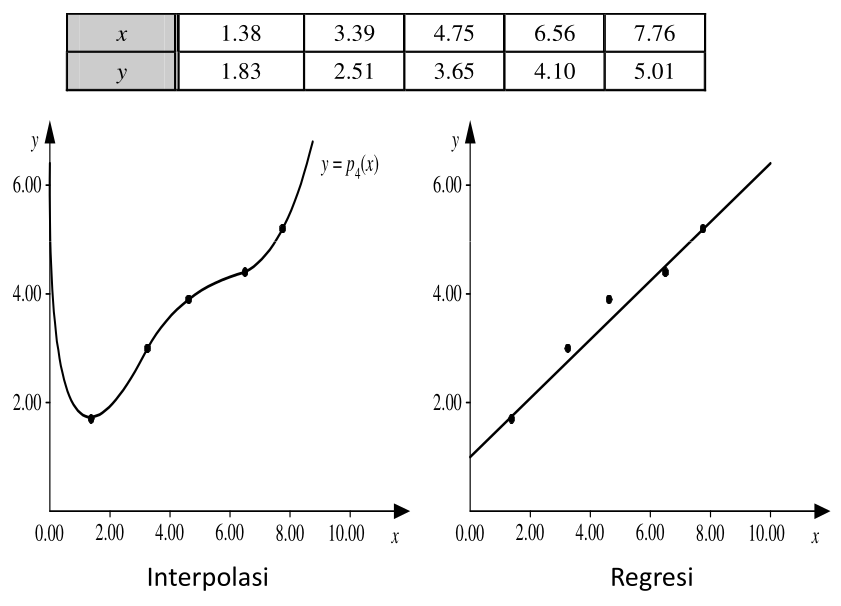
\includegraphics[width=0.6\linewidth]{img/img01}
	\end{center}
\end{frame}

\begin{frame}
	\begin{center}
		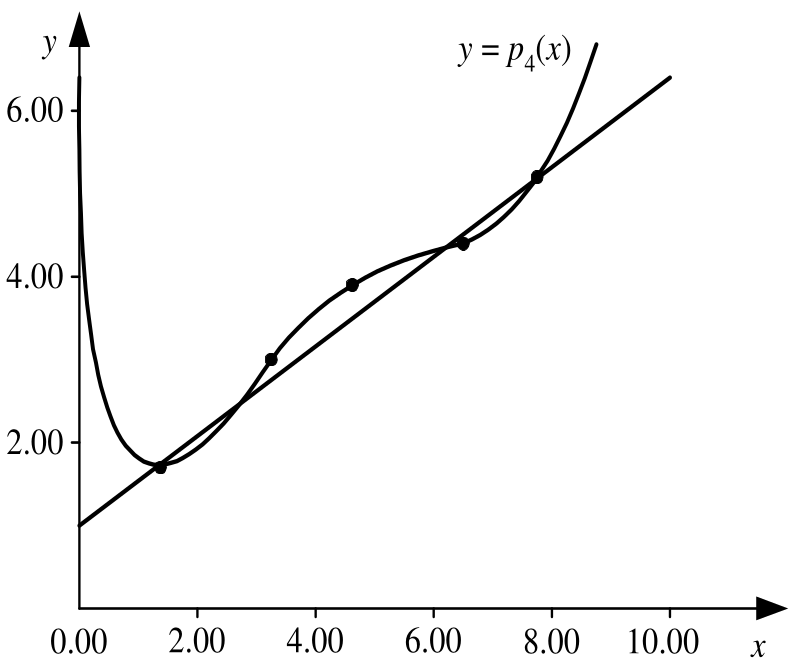
\includegraphics[width=0.5\linewidth]{img/img02}
	\end{center}
	\begin{itemize}
		\item Dari kedua pencocokan tersebut, terlihat bahwa garis lurus memberikan
hampiran yang bagus, tetapi belum tentu yang terbaik. Pengertian terbaik
di sini bergantung pada cara kita mengukur galat hampiran.
	\end{itemize}
\end{frame}

\begin{frame}
	\begin{itemize}
		\item Prinsip penting yang harus diketahui dalam mencocokkan
kurva untuk data hasil pengukuran adalah:
		\begin{itemize}
			\item Fungsi mengandung sesedikit mungkin parameter bebas
			\item Deviasi fungsi dengan titik data dibuat minimum.
		\end{itemize}
		\item Kedua prinsip di atas mendasari metode \textbf{regresi kuadrat
		terkecil}.
		\item Manfaat pencocokan kurva untuk data hasil pengukuran:
		\begin{enumerate}
			\item Bagi ahli sains/rekayasa: mengembangkan formula empirik
untuk sistem yang diteliti.
			\item Bagi ahli ekonomi: menentukan kurva kecenderungan
ekonomi untuk “meramalkan” kecenderungan masa
depan.
		\end{enumerate}
	\end{itemize}
\end{frame}

\section{Regresi Lanjar}

\begin{frame}
	\frametitle{Regresi Lanjar}
	\begin{itemize}
		\item Misalkan $ (x_i, y_i) $ adalah data hasil pengukuran. Kita akan
menghampiri titik-titik tersebut dengan sebuah garis lurus.
		\item Garis lurus tersebut dibuat sedemikian sehingga galatnya
sekecil mungkin dengan titik-titik data.
	\end{itemize}
	\begin{center}
		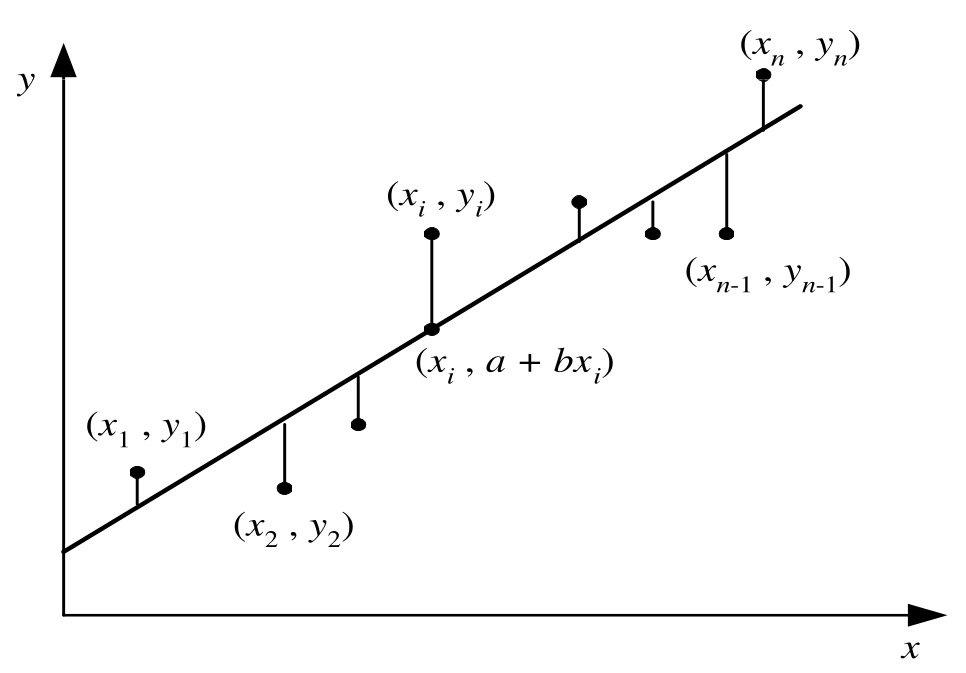
\includegraphics[width=0.5\linewidth]{img/img03}
	\end{center}
\end{frame}

\begin{frame}
	\begin{itemize}
		\item Karena data mengandung galat, maka nilai data sebenarnya,
$ g(x_i) $, dapat ditulis sebagai
		\begin{equation}
			g(x_i) = y_i + e_i\qquad i = 1, 2, \dots, n
		\end{equation}
		\item yang dalam hal ini, $ e_i $ adalah galat setiap data. Diinginkan
fungsi lanjar
		\begin{equation}
			f(x) = a + bx
		\end{equation}
		\item yang mencocokkan data sedemikian sehingga deviasinya,
		\begin{equation}
			r_i = y_i - f(x_i) = yi - (a + bx_i)
		\end{equation}
		minimum.
	\end{itemize}
\end{frame}

\begin{frame}
	\begin{itemize}
		\item Total kuadrat deviasi adalah
		\begin{equation*}
			R = \sum_{i=1}^{n}r_i^2 = \sum_{i=1}^{n}(y_i - a - bx_i)^2
		\end{equation*}
		\item Agar $ R $ minimum, maka haruslah
		\begin{align*}
			\frac{\partial R}{\partial a} &= -2\sum(y_i - a - bx_i) = 0 \\
			\frac{\partial R}{\partial b} &= -2\sum x_i(y_i - a - bx_i) = 0
		\end{align*}
		\item Untuk selanjutnya, notasi ditulis “$ \sum $” saja.
	\end{itemize}
\end{frame}

\end{document}
